\documentclass[10pt]{beamer}
\usepackage[spanish]{babel}
\usepackage[utf8]{inputenc}
\usepackage{color}
\usepackage{framed}
\usepackage{endnotes}
\usepackage{multicol}
\usepackage{graphicx}
\usepackage{caption}

\usetheme{Hannover}

\captionsetup[table]{font+=footnotesize, labelfont+=footnotesize}

\title{Exokernel}
\subtitle{An Operating System Architecture for \\  Application-Level Resource Managment}

\author{E. Mancuso\\ A. Mataloni\\ M. Miguel }

\date{16 de Junio de 2011}

\begin{document}
%-----slide------------------init--------------------
 \begin{frame}
  \titlepage
 \end{frame}
 \begin{frame}
  \tableofcontents
 \end{frame}
%----------------------------------------------------
\section{Introducción}
\subsection{Kernel Monolítico}
%-----slide------------------intro-------------------
\begin{frame}{Introducción}
La mayoría de los SO actuales utilizan kernels monolíticos, esto implica

\begin{itemize}
  \item Interfases de hardware genéricas
  \item Poca flexibilidad para la gran cantidad de aplicaciones existentes
  \item Implementaciones Ad-Hoc de abstracciones (Procesos, IPC, Archivos, etc)
  \item Las aplicaciones corren en máquinas virtuales cuya base con abstracciones de alto nivel
  \item Ocultar información del Hardware a la aplicación
  \item Frena la innovación en la implementación de abstracciones
\end{itemize}
\end{frame}

\subsection{Exokernel}
\begin{frame}

Es muy difícil implementar una abstracción que de un excelente rendimiento para toda aplicación existente y por ser desarrollada.\\[1em]

Por eso el exokernel propone cambiar la arquitectura monolítica por la siguiente \\[1em]

\begin{itemize}
  \item \textbf{Exokernel}: multiplexa los servicios de hardware de manera segura mediante primitivas de muy bajo nivel
  \item \textbf{Biblioteca SO}: Implementacion de abstracciones de alto nivel en espacio de usuario.
\end{itemize}
\end{frame}

\subsection{Arquitectura}
\begin{frame}
\begin{figure}[H]
\centering
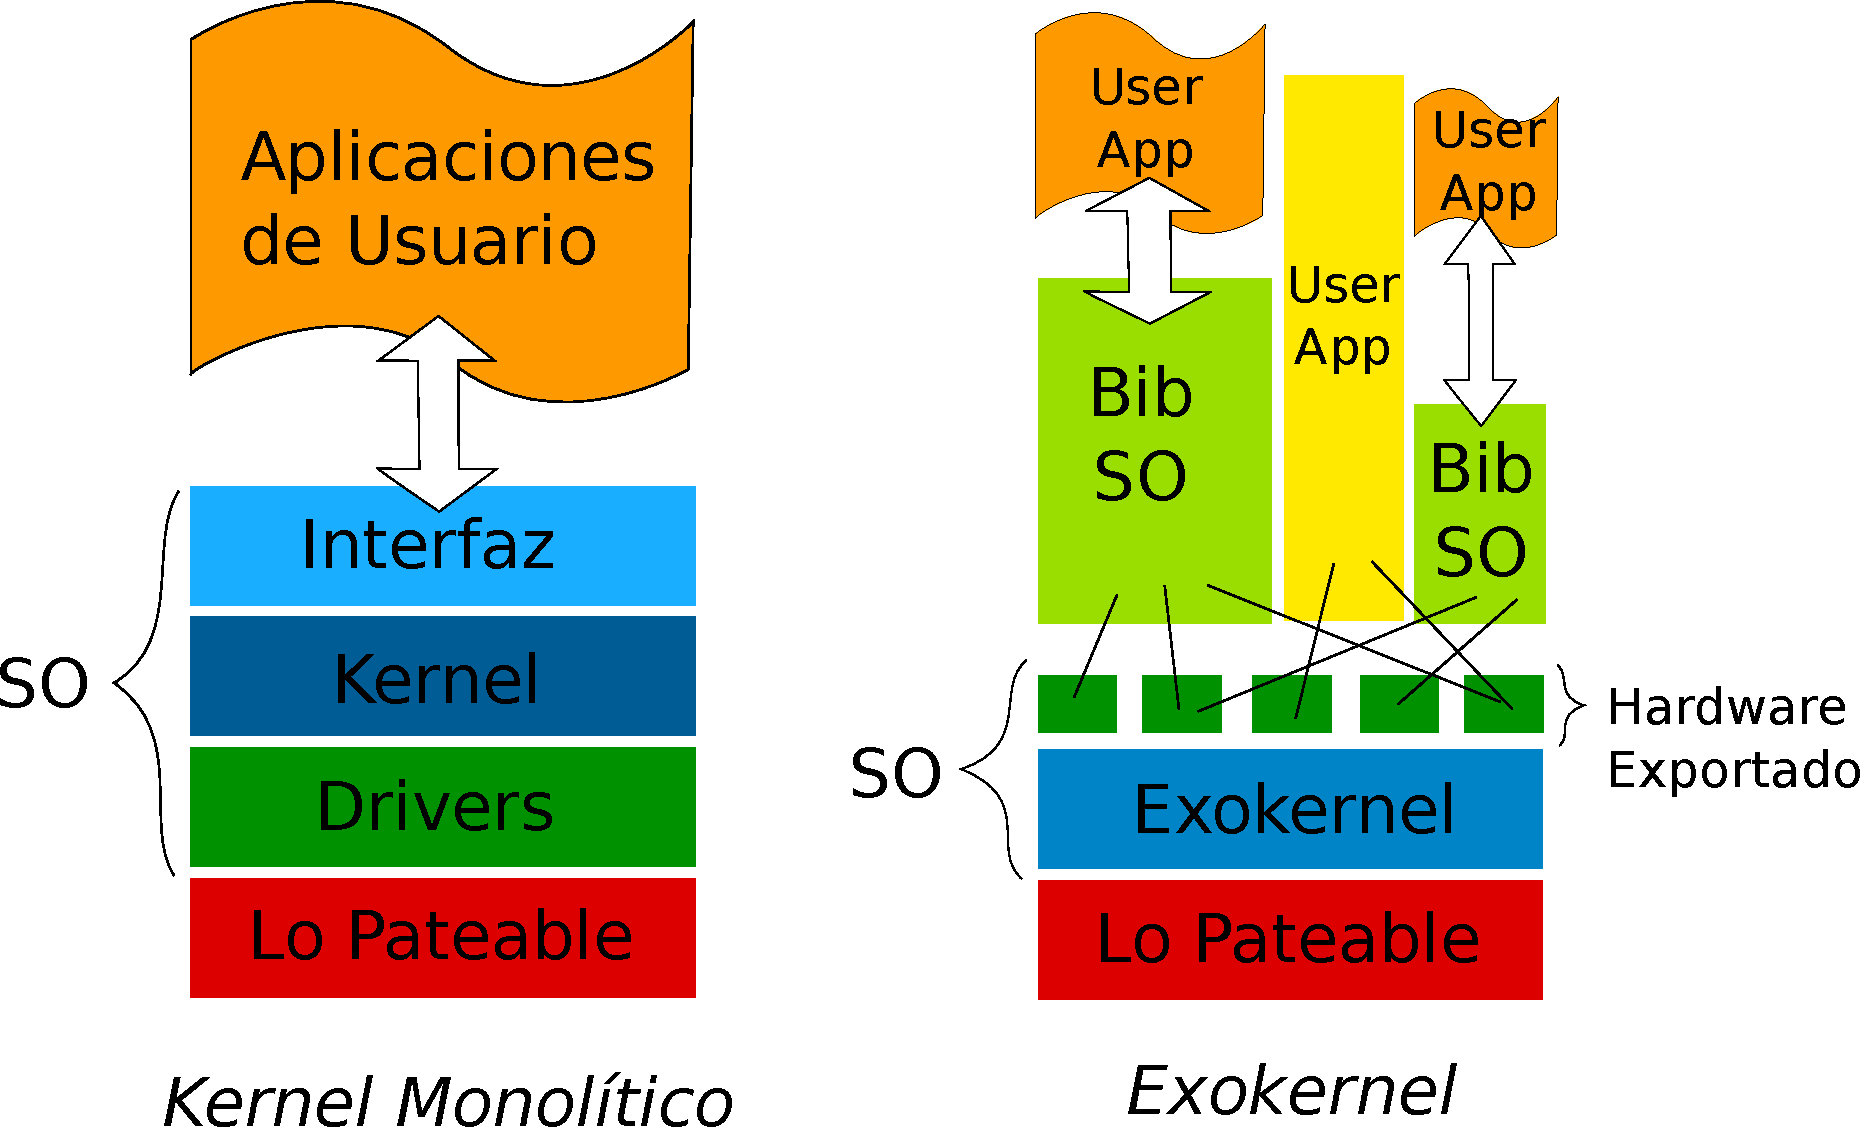
\includegraphics[scale=0.3]{grafico-kernel-exokernel.pdf}
\caption{Gráfico comparativo de los módulos en un kernel monolítico y un exokernel}
\end{figure}
\end{frame}

\subsection{Ventajas}
\begin{frame}
\begin{itemize}
  \item \emph{A menor nivel de la primitiva, más eficientemente puede esta implementarse}
  \item Interfaces más específicas
  \item Exportar el Hardware al usuario (programador de aplicaciones) en lugar de emularlo
  \item Se hace visible todo estado del hardware y se exportan las instrucciones privilegiadas (con protecciones)
  \item La interfaz se define en el espacio de usuario
  \item Controlar recursos desde nivel de usuario
  \item Las aplicaciones conocen mejor que el SO qué recursos necesitan y cómo administrarlos
\end{itemize}
\end{frame}

\section{Diseño}
\begin{frame}{Diseño}
Un \textbf{exokernel} se encarga de tres importantes tareas

\begin{itemize}
  \item Seguimiento de la asignación de recursos
  \item Garantizar la protección del uso de recursos o \textit{binding points}.
  \item Revocar el acceso a los recursos
\end{itemize}

\end{frame}


\subsection{Técnicas}
\begin{frame}
Para lograr implementar esta arquitectura hay que conocer las tres técnicas que utiliza el \textbf{exokernel} 

\begin{itemize}
  \item Secure bindings
  \item Visible resource revocation
  \item Abort protocol
\end{itemize}
\end{frame}


\subsubsection{Secure bindings}

\begin{frame}
\textbf{Secure bindings} \\[2em]

Es un mecanismo de protección que desacopla autorización del uso real de un recurso.\\[1em]

Las bibliotecas de Sistema Operativo pueden unirse o \textit{'bindiarse'} al Hardware para tener un mayor control sobre los eventos. \\[1em]  
La autorización se realiza sólo en el \textit{binding time}, esto permite separar la administración de la protección.\\[1em]

El \textbf{exokernel} interviene en todos los accesos a recurso.

\end{frame}

\subsubsection{Visible resource revocation}

\begin{frame}
\textbf{Visible resource revocation} \\[2em]

Como parte del concepto de \emph{que el usuario sabe manejar sus recursos mejor}, se permite a las \textbf{bibliotecas de sistema operativo} participar en el protocolo de revocación de recursos.\\[1em]

Esto significa que, cada vez que el \textbf{exokernel} necesita que se liberen recursos, el protocolo para lograr la liberación implica una conversación entre el kernel y a \textbf{biblioteca OS}. En el mismo, se hace un pedido de liberación a desde el kernel al nivel aplicación.

\end{frame}


\subsubsection{Abort protocol}

\begin{frame}
\textbf{Abort protocol} \\[2em]

Es un protocolo para romper, a la fuerza, \textit{secure bindings} con las \textbf{bibliotecas de sistema operativo} que no cooperan o fallan al responder una solicitud de revocación.\\[1em]

El \textbf{exokernel} rompe todos los \textit{secure bindings} existentes con el recurso e informa a la \textbf{biblioteca de sistema operativo}. Ésta acción es registrada en un \textit{vector de recuperación} y la biblioteca recibe una excepción de \textbf{recuperación} para actualizar a quienes utilizan el recurso.

A las \textbf{bibliotecas de sistema operativo} se les asegura un mínimo de recursos que no le serán revocados. 

\end{frame}


\section{Experimentos}

\begin{frame}{Experimentos}
Para ver que esto efectivamente puede suceder, se implemento \textbf{Aegis} un exokernel y \textbf{ExOS}, una biblioteca de sistema operativo que implementa las abstracciones más importantes de los sistemas operativos. 

Los experimentos prueban estas hipótesis

\begin{itemize}
  \item Los \textbf{Exokernels} pueden ser muy eficientes
  \item La multiplexación segura de hardware se puede implementar de manera eficiente a bajo nivel.
  \item Las abstracciones de SO tradicionales se pueden implementar eficientemente a nivel de aplicación.
  \item Las aplicaciones pueden crear implementaciones de estas abstracciones con propósito específico.
\end{itemize}
\end{frame}

\subsection{Excepciones}

\begin{frame}
\textbf{Excepciones}\\[2em]
\begin{table}
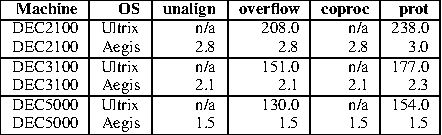
\includegraphics[scale=0.8]{grafico-excepciones.pdf}
\caption{Tiempo de envío de excepciones en \textbf{Aegis} y \textbf{Ultrix} (tiempos en milisegundos).}
\end{table}

En \textbf{Aegis}, al producirse una excepción, el estado se guarda en un área de memoria ya acordada con el usuario, con accesos directos a memoria física. Esto evita \emph{TLB misses}.

Luego se ejecuta el controlador de interrupciones de la aplicación, dejando a su disposición la información necesaria para que pueda reconstruir el estado necesario y vuelva a ejecutar sin pasar nuevamente por el kernel. 
\end{frame}

% \captionsetup[table]{font+={footnotesize}}
\subsection{IPC}

\begin{frame}
\textbf{IPC} \\[2em]
\begin{table}
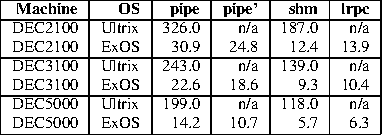
\includegraphics[scale=0.8]{grafico-ipc.pdf}
\caption{Comparativas de implementaciones de \textbf{IPC} en \textbf{ExOS} sobre \textbf{Aegis} y \textbf{Ultrix} (tiempos en milisegundos). Para pipe y memoria compartida las mediciones son unidireccionales, para LRPC es bidireccional.}
\end{table}
En estos experimentos se hace una prueba de ping-pong entre dos procesos actualizando un contador. \textbf{pipe'} es una implementación más eficiente de \textbf{ExOS} de pipes. En \textbf{lrpc} se mide el tiempo de hacer una llamada remota, actualizar un contador en otro espacio de direcciones y volver al contexto original. 
\end{frame}

\subsection{Memoria virtual}

\begin{frame}
 \textbf{Memoria virutal} \\[2em]
\begin{table}
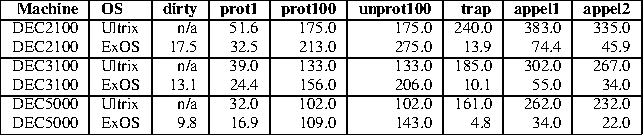
\includegraphics[scale=0.8]{grafico-vm.pdf}
\caption{Comparativa de tiempos de operaciones de memoria virtual en \textbf{ExOS} y \textbf{Ultrix} (Tiempos en milisegundos). \textbf{appel1} y \textbf{appel2} son benchmarks de \emph{Appel and Li} y el tiempo presentado promediado por página.}
\end{table}
\end{frame}

\subsection{Flexibilidad}

\begin{frame}
\textbf{Flexibilidad} \\[2em]
Se presentan los beneficios de trabajar con distintas implementaciones de la mismas abstracciones. 
\begin{table}
 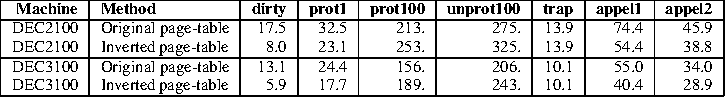
\includegraphics[scale=0.8]{grafico-pages.pdf}
\caption{Operaciones de memoria virtual usando distintas estructuras de tablas de página (tiempos en milisegundos).}
\end{table}

\begin{table}
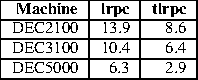
\includegraphics[scale=0.8]{grafico-tlrpc.pdf}
\caption{Comparación de ejecuciones de \emph{lightweight remote procedure call} contra \emph{trusted lightweight remote procedure call} (tiempos en milisegundos).}
\end{table}
\end{frame}

\section{Conclusión}

\begin{frame}{Conclusión}
 \begin{itemize}
  \item El \textbf{exokernel} permite crear abstracciones de alto nivel especializadas para cada tipo de aplicación. Esto lleva a una mejora en rendimiento y flexibilidad.
  \item Los experimentos realizados sobre las implementaciones \textbf{ExOS} y \textbf{Aegis} demostraron las hipotesis.
  \item Basado en los resultados, se concluye que la arquitectura del \textbf{exokernel} es una estructura viable para la implementación de sistemas operativos extensibles y con muy buen rendimiento.
\end{itemize}
\end{frame}



%----------------------------------------------------
\end{document}